\documentclass{article}
\usepackage{hyperref}
\usepackage{listings}
\usepackage{graphicx}
\usepackage[backend=bibtex]{biblatex}
\addbibresource{ug.bib}

\title{LoFASM Pulsar Search with PRESTO}
\author{Keith E. Boehler Jr.}
\date{}
\begin{document}
\maketitle
   Hello world! We are using Scott's PRESTO \textcite{Ransom01}

\section{Background}

\section{Tools Used}
\subsection{bbx to sigproc}
This program was made to fill the gap between formats that PRESTO understands and LoFASM generated files. The steps taken to convert between bbx filterbank and sigproc filterbank are based on the documentation by Dunc Lorimer \textcite{LorimerSigproc}.
\begin{itemize}
	\item The function \texttt{prepHeader} maps bbx header values to their corresponding keys in sigproc. Many are a 1-1 map while the hard coded ones are there as place holders. 
	\item \texttt{fbTranscribe} orders the data to sigproc standards. The bbx format has a two dimensional array of time and frequency; the frequencies are arranged from low to high. Sigproc expects them to be in reverse order.   
	\item The script has a few flags to manage inputs and modify outputs. The first is a path used to pass the file to be converted. Next are flags that modify the range of frequencies to be used in the out put. Since LoFASM is less sensitive on the fringes it takes the center 50Mhz bandwidth by default.
\end{itemize}
Typical use is as follows: \begin{lstlisting}[language=bash]
$ python bbx2sigproc.py -p /path/to/file.bbx -l 20 -h 80
\end{lstlisting}
This should generate a filterbank file named after the input, \texttt{file.fil}, with a span between 20Mhz to 80Mhz in the directory where it was run.

\subsection{lofasmio}

\section{Installing PRESTO}
The instructions here are based on those by Scott Ransom's Install page on github as well as other tips found on the internet. The following will be centered on using Ubuntu 20.04. Tips for macOS Mojave will be provided as well. 
\subsection{Prerequisites}
\begin{enumerate}
   	\item GNU gcc with gfortran
    \item For glib: csh autoconf meson libglib2.0-dev
    \item For cfitsio: libcfitsio-bin libcfitsio-doc libcfitsio-dev
    \item For PRESTO: libpng.dev zlib1g-dev
    \item For FFTW3: libfftw3-bin libfftw3-dev
    \item Python 2.7 with virtual env. Anaconda works well. 
\end{enumerate}
   
\subsection{FFTW 3}
    This one is rather straight forward. 
\begin{enumerate}
    \item At the time of this writing the latest version is 3.3.8 and can be downloaded \href{http://www.fftw.org/download.html}{from this link}
    item \noindent Once the source has been downloaded it can be unpacked using the command:
	\begin{lstlisting}[language=bash]
	    $ tar -zx fftw-x.x.x.tar.gz 
	\end{lstlisting}
    (Will need to replace the x.x.x with the current version number). And enter the unpacked directory.
    \item \noindent After that we need to configure. According to Scott there are some suggested flags if you are
    	using an Intel chip, which I am. So my command will look like: 
	\begin{lstlisting}[language=bash]
	./configure --prefix=$HOME \
	--enable-shared --enable-single \
	--enable-sse --enable-sse2 --enable-avx \
	--enable-avx2 --enable-fma
	\end{lstlisting}
	\item \noindent Followed by: \begin{lstlisting}[language=bash]
	$ make
	\end{lstlisting}
	\item \noindent Followed by: 
	\begin{lstlisting}[language=bash]
	$ make check
	\end{lstlisting}
	\item \noindent Followed by: 
	\begin{lstlisting}[language=bash]
	$ make install
	\end{lstlisting}
	\item \noindent Followed by:
	\begin{lstlisting}[language=bash]
		 $ make installcheck
		\end{lstlisting}
    \end{enumerate}
    Due to the fact that we used \$HOME in our prefix we should have /bin /include and other directories
    being made in our home directory. This will help later when we are making our environment variables
    as the location of configure files and executable will be in more standard location.
    
\subsection{PGPLOT}
    This one is a bit involved, so I recommend brewing your favorite cup of Joe before getting started. This
    portion is based on the PGPLOT’s instructions for all UNIX systems. 
\begin{enumerate}
    \item \noindent I downloaded my source for PGPlot from \href{ftp://ftp.astro.caltech.edu/pub/pgplot/pgplot5.2.tar.gz}{here, version 5.2.}. And untarred with: 
    \begin{lstlisting}[language=bash]
    $ tar -xzvf pgplot5.2.tar.gz
    \end{lstlisting}
     At this point it is prudent to create what the pgplot unix instructions call the target directory, that is where we will install. I find it to be clear to rename the directory we just unpacked to \texttt{pgplot\_src} and the actual install directory to be \texttt{pgplot}. 
    \item Copy the drivers list from the source directory (\texttt{pgplot\_src}) into our install directory (\texttt{pgplot}). If you are inside the install directory here is a snippet: \noindent
    \begin{lstlisting}[language=bash]
    $ cp ../pgplot_src/drivers.list .
    \end{lstlisting} 
    \item Using any text editor open the drivers file. Uncomment the needed drivers by removing the `` ! '' from the needed line. It is recommended to only uncomment the needed drivers. For PRESTO we at a minimum need the postscript (those with PS in the name) and xwindow (xw and xserver). And save the changes. 
    \item Create the Makefile. This step can be somewhat involved so a fresh pot of coffee is needed to lift spirits. While the below is going to be centered for Ubuntu 20.04 I do have some tips for installing on macOS Mojave. I used homebrew to install xquartz (an xserver for mac), gcc (for gfortran and the c compiler.), and there is also a special configuration file that can be found \href{http://mingus.as.arizona.edu/~bjw/software/pgplot_macosx_conf.tar}{at this location}. Otherwise the following should be similar:
\begin{enumerate}
    \item Run the makemake script with the following template: \texttt{path2/pgsrc/makemake path2/pgsrc Ostype fortran/cc}. That is to say while in your target directory run stuff in your source directory. Select if you are using linux and a C-Compiler and Fortran compiler. It is worth noting that we will edit the resulting Makefile with the compilers we will actually use. My command looks like this: \begin{lstlisting}[language=bash]

$./pgplot_src/makemake ../pgplot_src/ linux g77_gcc
    \end{lstlisting}
    \item Enter the makefile and change the \texttt{FCOMPL} to \texttt{gfortran} (install if you dont have it at this point. Also on macOS should change the C compiler to a gcc one). Then type \texttt{make}. My install of Ubuntu is fresh so it was also missing \texttt{libx11-dev} (X11/Xos.h: No such file or directory ← Error). Here is what a successful run looks like: Figure \ref{fig:pgplot-make}.     			
\begin{figure}[h]
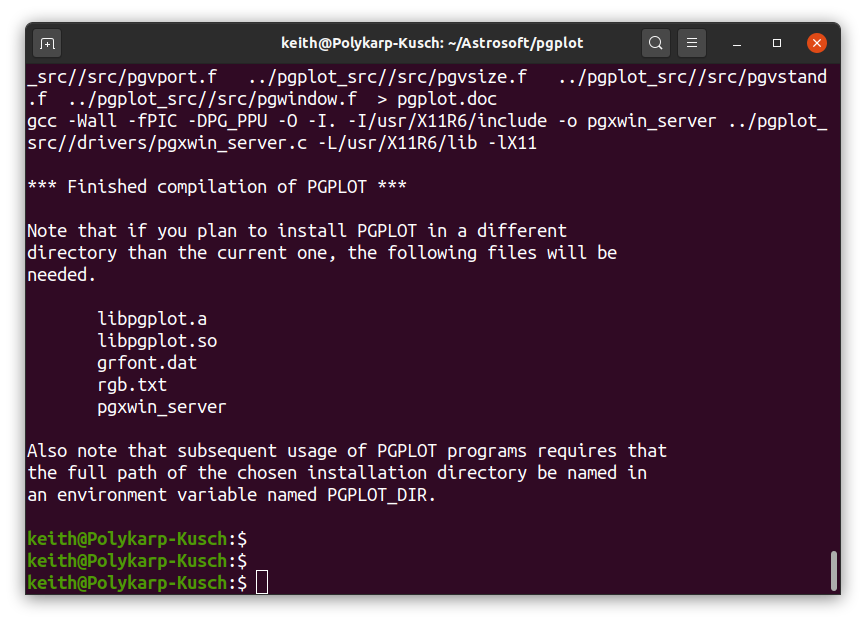
\includegraphics[width=\linewidth]{Images/sucesfful-pgplot-make.png}
\caption{Successful PGPlot make}
\label{fig:pgplot-make}  			
\end{figure}
    \item Enter: \texttt{\$ make cgp} \ref{fig:pgplot-make-cpg}
\begin{figure}[h]
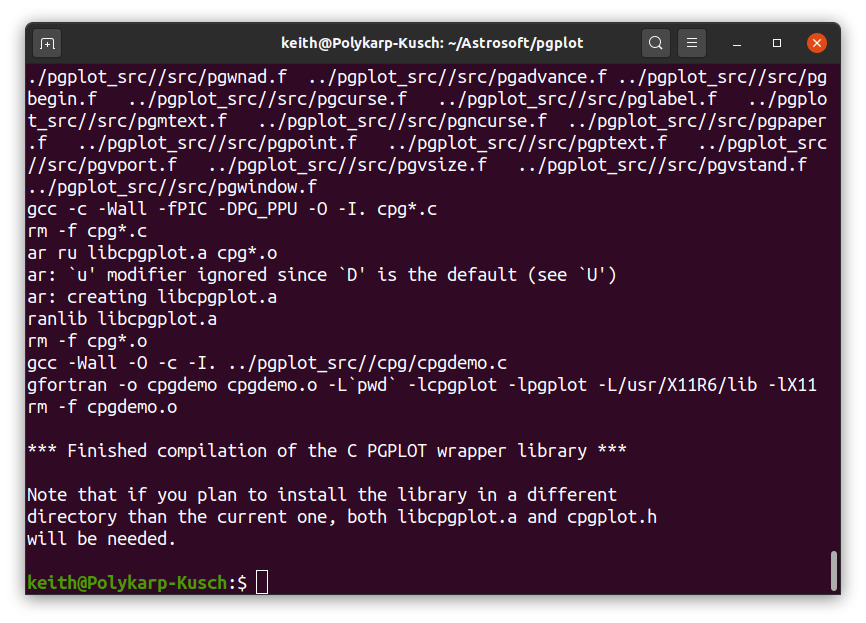
\includegraphics[width=\linewidth]{Images/sucesfful-pgplot-make-cgp.png}
\caption{Successful PGPlot make cpg}
\label{fig:pgplot-make-cpg}  			
\end{figure}
    \item Enter: \texttt{\$ ld -shared -o libcpgplot.so --whole-archive libcpgplot.a}
    			
    			
    \item At this point we should set our environment variables 
\footnote{I like to keep a file in my home directory called \texttt{.bash\_astro}. In it i have a variable called \texttt{ASTROSOFT} that points to where i am installing my programs. For example my \texttt{LD\_LIBRARY\_PATH} will be defined as: \texttt{export LD\_LIBRARY\_PATH=\$ASTROSOFT/pgplot:\$LD\_LIBRARY\_PATH}. The word \texttt{export} tells bash this is environment variable. The \texttt{\$} is used to envoke other variables. The \texttt{':'} is to re-appending any previous \texttt{LD\_LIBRARY\_PATH}.}. 
    			This will allow our shell to find shared objects, executables, and device outputs. We will need the \texttt{PGPLOT\_DIR=/path/to/pgplot}; this should have the files \texttt{grfont.dat} and \texttt{rgb.txt}. We will also need a \texttt{LD\_LIBRARY\_PATH} that should point to the file \texttt{libpgplot.so}, If you compiled from source like we did in this example it should be in the same big directory. Finally we can set the \texttt{PGPLOT\_DEV=/XWINDOW} to default to outputting to an xwindow. 
    			
    \item In principle we are done. Now lets test our work by running the demo programs \ref{fig:sucesfful-pgplot-install}.  
\begin{figure}[h]
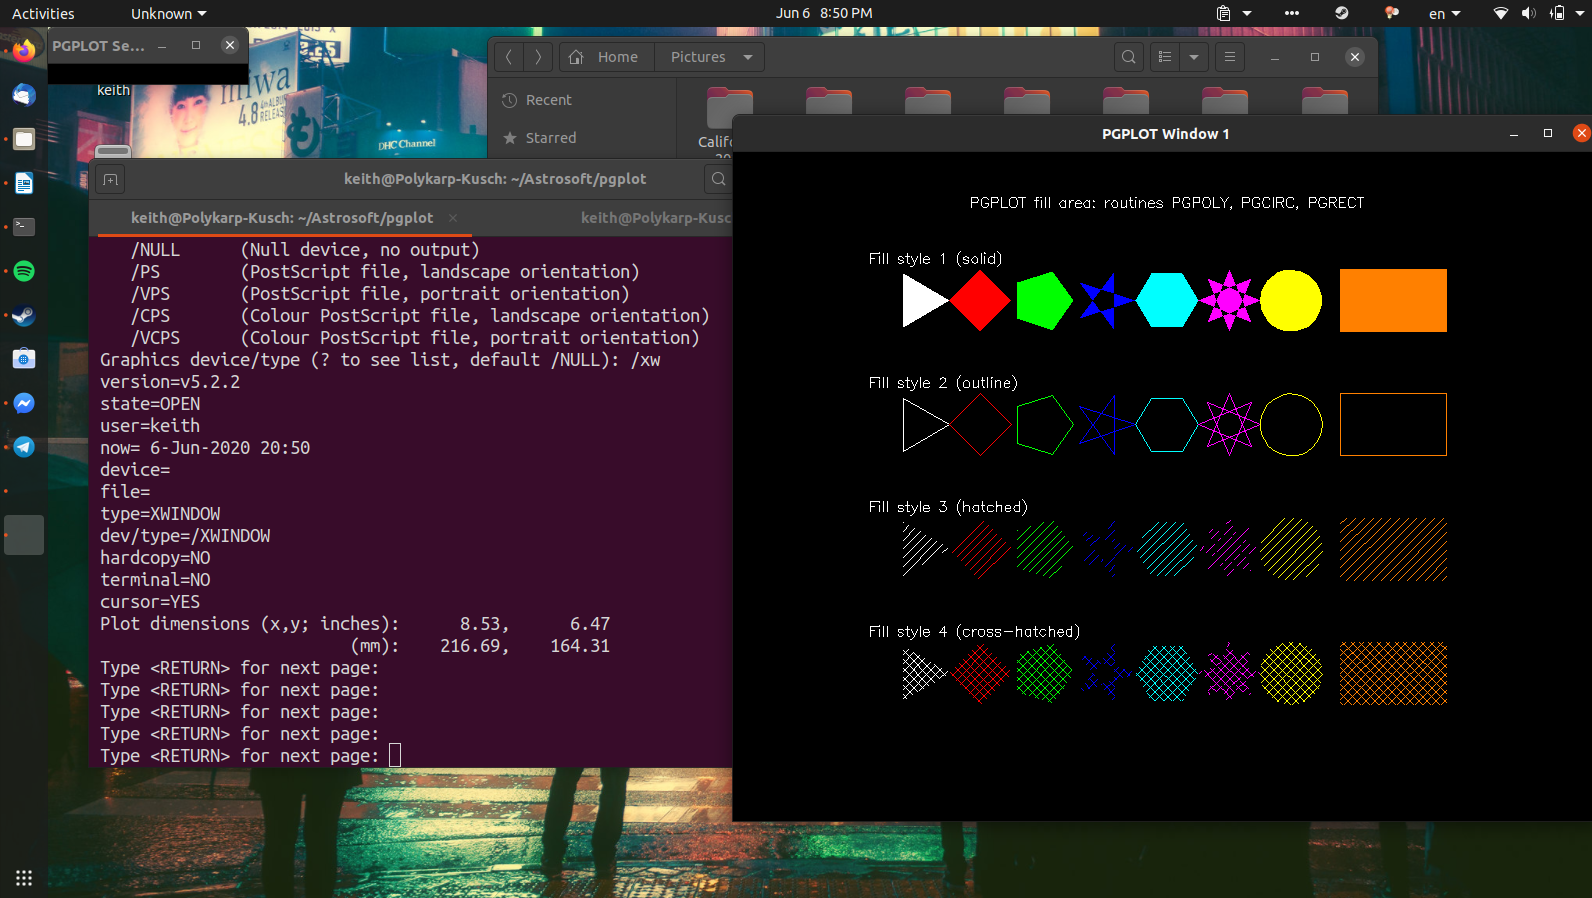
\includegraphics[width=\linewidth]{Images/sucesfful-pgplot-install.png}
\caption{Run them with ./pgdemo1}
\label{fig:sucesfful-pgplot-install}  			
\end{figure}    	
\end{enumerate}   		
\end{enumerate}
    	
\subsection{TEMPO}
\begin{enumerate}
    \item Cloning the source from \href{git://git.code.sf.net/p/tempo/tempo}{git.}
    \item run \texttt{./prepare}
    \item run: \noindent \begin{lstlisting}[language=bash]
    $ ./configure --prefix=$HOME
    \end{lstlisting} 
    \item run \texttt{make}
    \item run \texttt{make install}
\end{enumerate}
\subsection{GLIB}
   This resource from \href{http://www.linuxfromscratch.org/blfs/view/svn/general/glib2.html}{was found to be helpful.}
\begin{enumerate}
    \item We will need the \texttt{Libglib2.0-dev} libraries and the source from gnome \href{http://ftp.gnome.org/pub/gnome/sources/glib/2.64/glib-2.64.3.tar.xz}{as of writting latest version is 2.64}. Un tar once the file has been downloaded.  
    \item Create a directory called build and enter it.
    \item use meson with \begin{lstlisting}[language=bash]
    $ meason --prefix=$HOME -Dman=true -Dselinux-disabled
    \end{lstlisting}
    \item then type \texttt{ninja}
    \item followd by \texttt{sudo ninja install}
\end{enumerate}
         
\subsection{CFITSIO}
\begin{enumerate}
    \item Download the latest version from \href{http://heasarc.gsfc.nasa.gov/FTP/software/fitsio/c/cfitsio-3.48.tar.gz}{nasa} and untar.
    \item Run: \begin{lstlisting}[language=bash]
    $ ./configure --prefix=$HOME 
    \end{lstlisting}
    \item \texttt{make}
    \item \texttt{make install}
\end{enumerate}
\subsection{Python}
For the current relese of presto we will need python 3.7. Tho similar steps are to be taken with python 2.7 for presto 2.2. 
\begin{enumerate}
    \item Download \href{Anaconda 3}{https://docs.anaconda.com/anaconda/install/linux/} and run the install script. \begin{lstlisting}[language=bash]
$ bash ~/Download/Anaconda-whateverVersionNumber.sh
\end{lstlisting}
There is a sha256 code that can be verified aswell for security. 
    \item It is good practice to always work witha virtual enviroment when using python. Anaconda supports this with: \begin{lstlisting}[language=bash] 
$ conda create --name ur-name python=3.7
\end{lstlisting} 
A newer version of python 3.8 was tried, but the author found much greif.
The enviroment can be activated with \texttt{conda activate ur-name}. You should see your terminal now have that name in parenthasis in the begining of the prompt.
    \item Needed Moduals: \begin{lstlisting}[language=bash]
    # for just presto
    $ conda install numpy scipy
    # if using the lofasm tools also
    $ conda install matplotlib astropy
    \end{lstlisting}
\end{enumerate}
\subsection{PRESTO}
\begin{enumerate}
    \item Add presto to our bash astro file (where we placed the enviroment variables for PGPlot). It should point to the top level of the presto directory. Example with other variables that need to be set: \begin{lstlisting}[language=bash]
    export PRESTO=$ASTROSOFT/presto
    export LD_LIBRARY_PATH=$PRESTO/lib:$LD_LIBRARY_PATH 
    export PATH=$PRESTO/bin:$PATH
    # Do not add if using Presto 3
    export PYTHONPATH=$PRESTO/lib/python 
    \end{lstlisting}
    Don't forget to \texttt{source ~/.bash\_astro} in order to take effect. If you are checking out an older version of presto then the \texttt{PYTHONPATH} variable is needed and the rest of the isntall is basicly the same.  
    \item Go into the \texttt{PRESTO/src} directory and run:  \begin{lstlisting}[language=bash]
    $ make makewisdom 
    \end{lstlisting}
    This command may take a while to run. 
    \item Type \texttt{make prep}.
    \item Followed by \texttt{make}.
    \item Python 3.7, its moduals, and virtual enviorment should be loaded.
    \item In the \texttt{\$PRESTO/setup.py} file add \texttt{/opt/local/include} to the \texttt{include\_dirs}. Also add \texttt{gfortran} to the \texttt{ppgplot\_libraries}.
    \item Install with: \begin{lstlisting}[language=bash]     
    $ cd $PRESTO ; pip install .
        \end{lstlisting}
        If errors are found it maybe needed to modify the \texttt{setup.py} file. Add ``gfortran'' into the \texttt{ppgplot\_libraries} line. 
        Here is the end result\ref{fig:Presto-Install}. 

    \item Test the instalation: 
        \begin{enumerate}
        \item Download Scott Ransom's PRESTO \href{https://www.cv.nrao.edu/~sransom/PRESTO_search_tutorial.pdf}{toutorial}.
        \item Download the test data from the link in the slides
        \item Run the \texttt{readfile} and \texttt{prepfold} commands. Ensure that they complete succsesfully at a minimum. Going over the rest of the document is also a good overview of the tools included.
        \end{enumerate}
    \item Find Pulsars, Good Hunting!
\end{enumerate}

\begin{figure}
	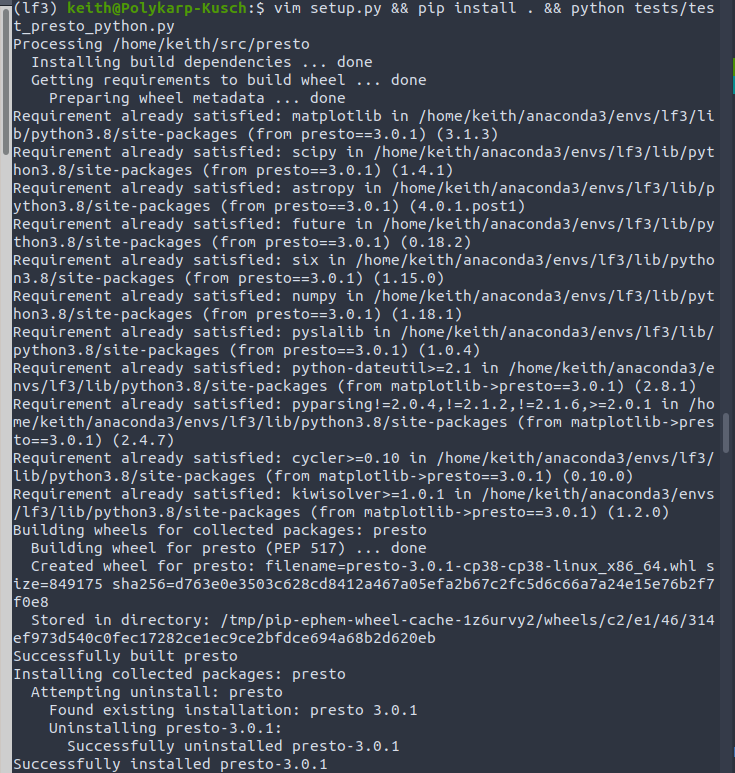
\includegraphics[width=\linewidth]{Images/PRESTO3_install.png}
	\caption{Successful Presto Install with unit tests}
	\label{fig:Presto-Install}  			
\end{figure}

\printbibliography


\end{document} 
